\chapter{Results}

\section{UI Implementation}

\subsection{Parsing template document}
The system provides a user-friendly interface for adding new templates, as shown in Figures 4.1 below. The process includes filling in template information, uploading a .docx file, and saving it to the template management list. Once uploaded successfully, templates files are stored on Supabase and can be selected later when generating reports.

The Template page (Figure 4.1) displays a list of all active templates, including the ability to Edit or Delete them. This helps the admin easily manage templates used for report generation.

\textbf{Steps to add new template document}

\begin{enumerate}
    \item Click the Create button on the Template Management page to open the Create New Template modal (Figure 4.2).  
    \item Enter the template name and description, choose the file to upload, then select template type (Form or Report), and status (Active or Draft) as the Figure 4.3.
    \item Press the blue Upload File button to upload the document to Supabase. A success message “File uploaded successfully!” will appear if the upload is successful (Figure 4.4).
    \item After that, press the blue Create Template button to save the template.
    \item The new template will appear in the Template Management list (Figure 4.5), ready to be used in report creation.
    
\end{enumerate}
\begin{figure}[h]
\centering
    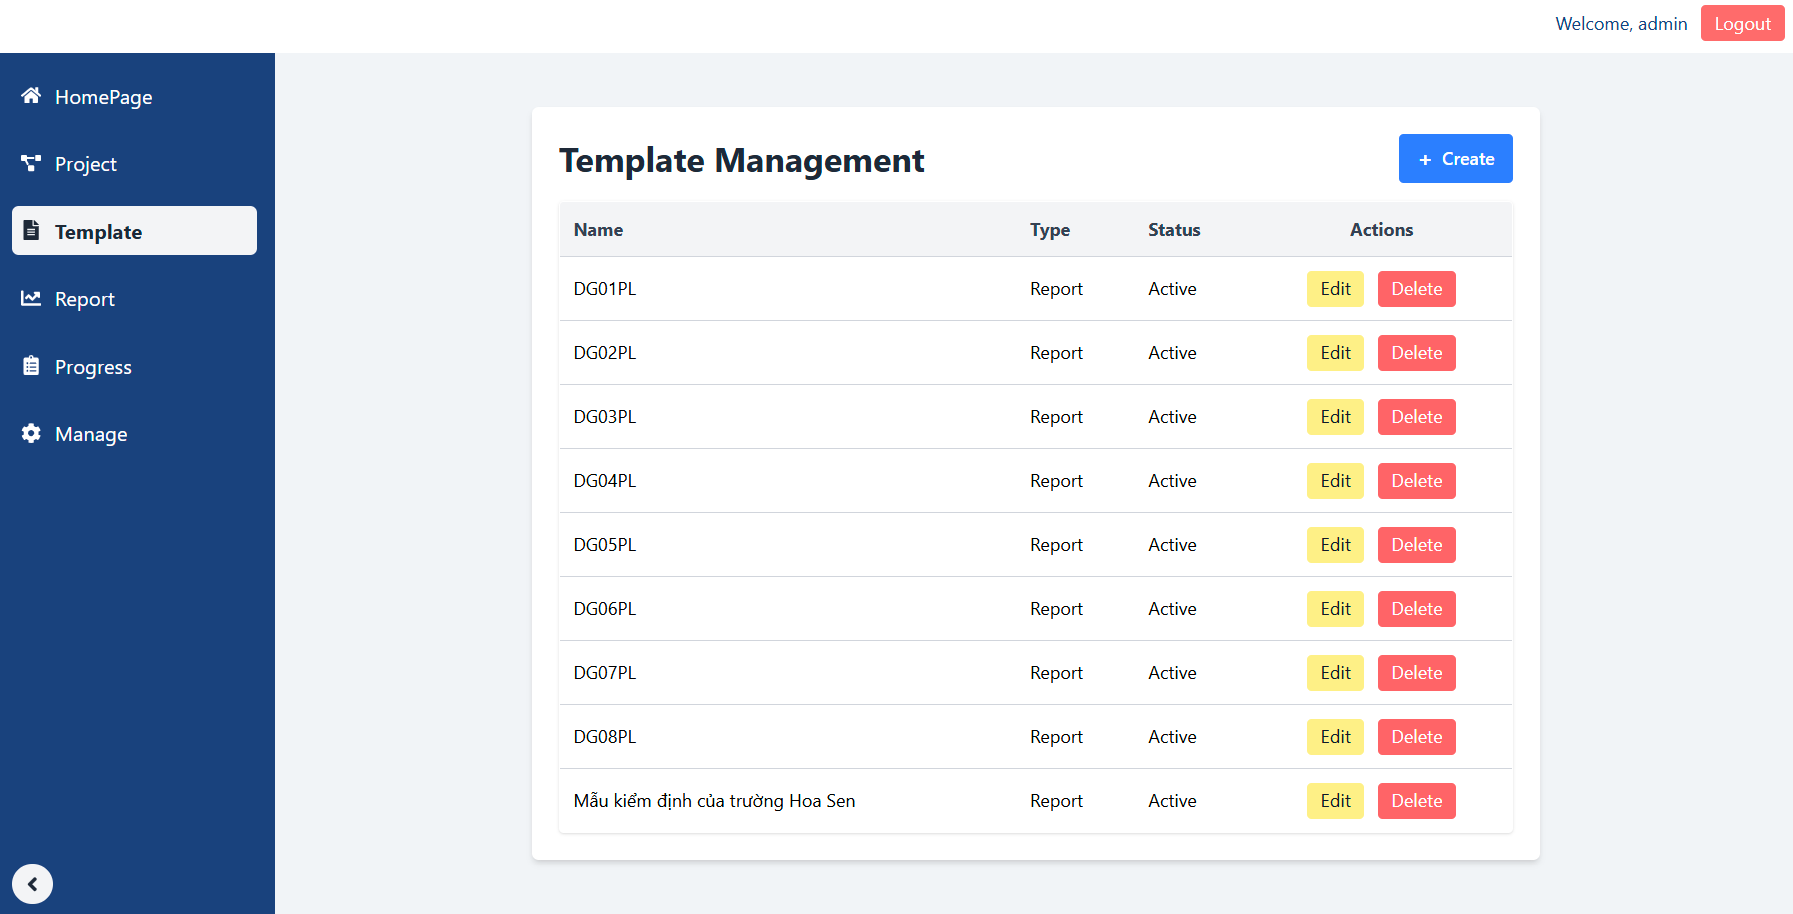
\includegraphics[width=0.5\textwidth]{images/template_page.png}
    \caption{Template page} 
    \label{fig:template}
\end{figure}
\begin{figure}[h]
\centering
    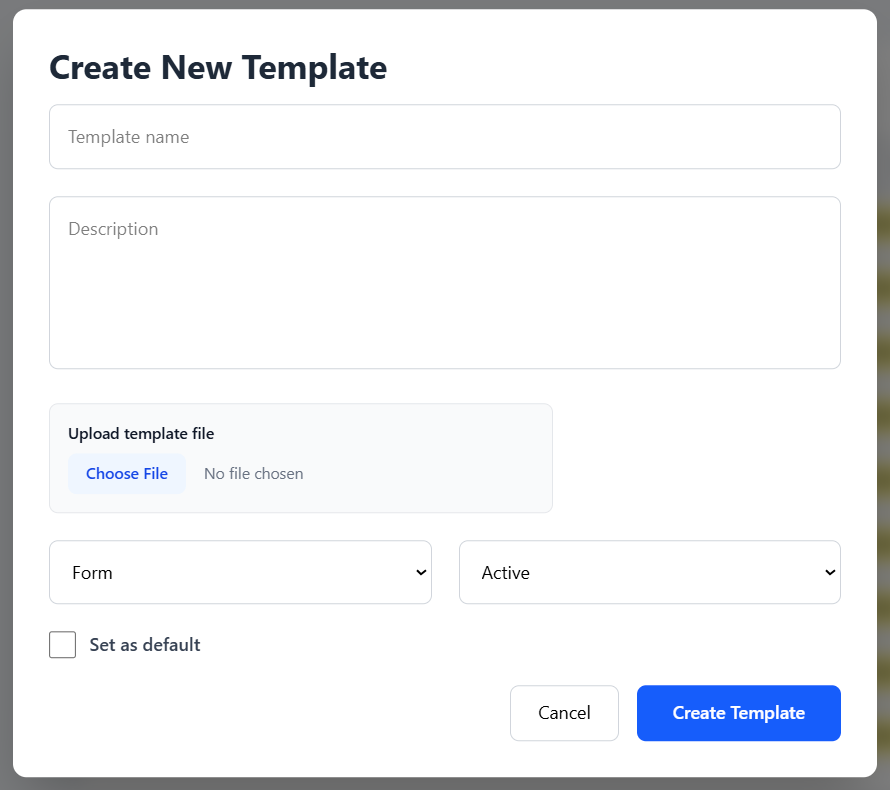
\includegraphics[width=0.5\textwidth]{images/template_modal.png}
    \caption{Template Modal pop-up} 
    \label{fig:template_modal}
\end{figure}

\begin{figure}[h]
\centering
    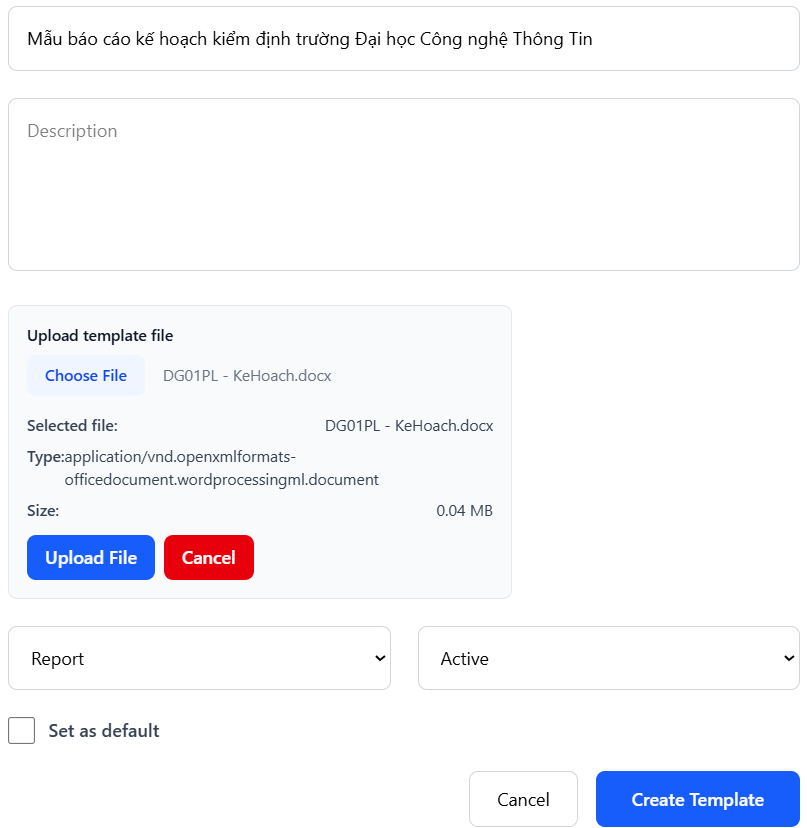
\includegraphics[width=0.5\textwidth]{images/adding template.png}
    \caption{The Template file import} 
    \label{fig:template_modal}
\end{figure}

\begin{figure}[h]
\centering
    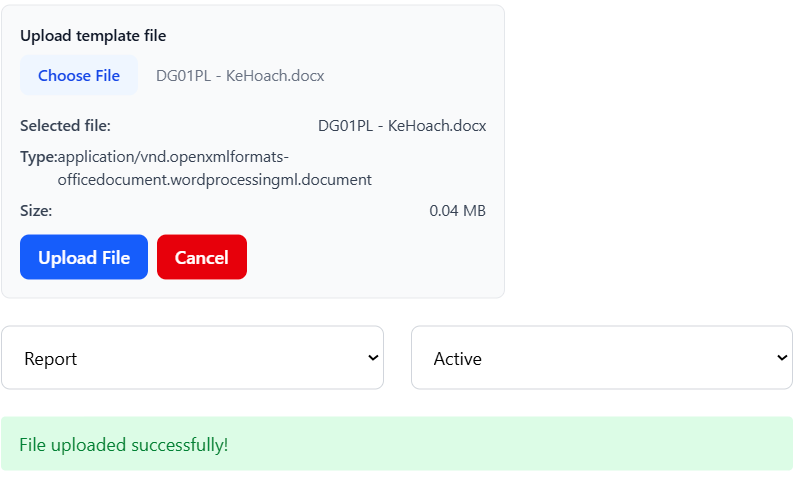
\includegraphics[width=0.5\textwidth]{images/adding_sucess.png}
    \caption{The Template file  has been added} 
    \label{fig:adding_sucess}
\end{figure}

\begin{figure}[h]
\centering
    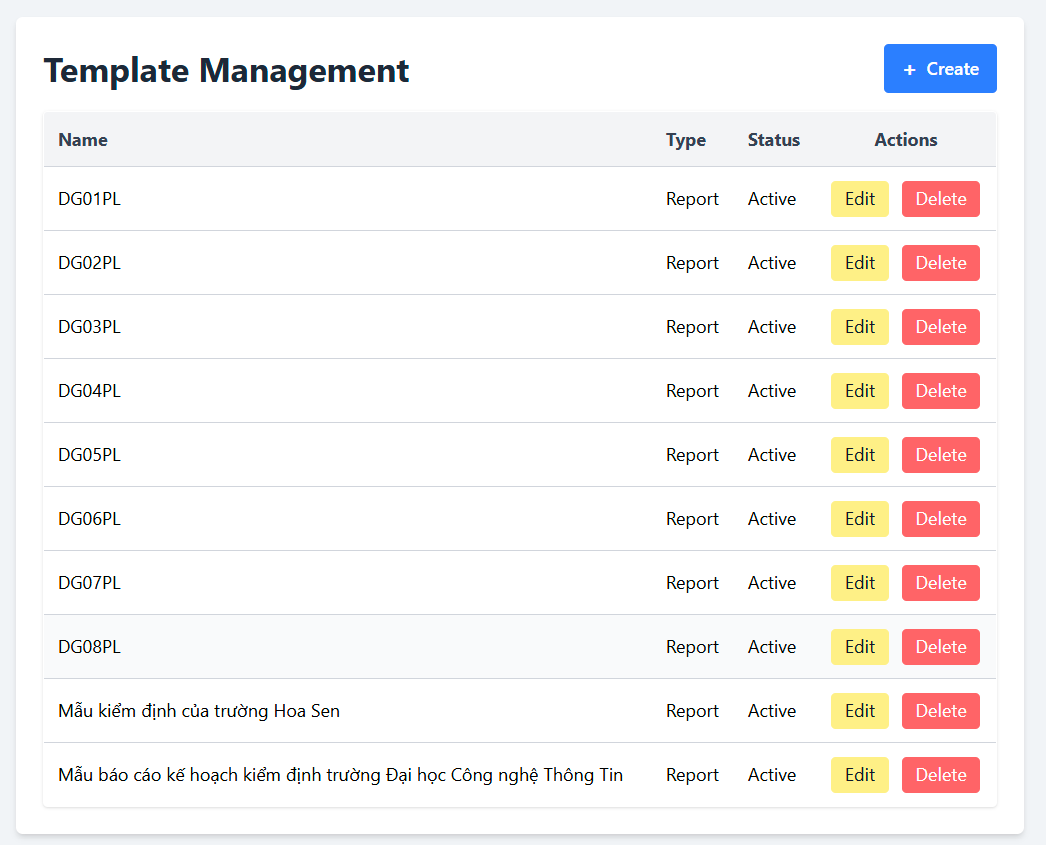
\includegraphics[width=0.5\textwidth]{images/template_sucess.png}
    \caption{The Template successfully created} 
    \label{fig:template_sucess}
\end{figure}
This process ensures that templates are consistently stored, version-controlled, and easily accessible for creating new documents, contributing to the overall usability and scalability of the accreditation support system.

\subsection{Create new document}

\begin{figure}[h]
\centering
    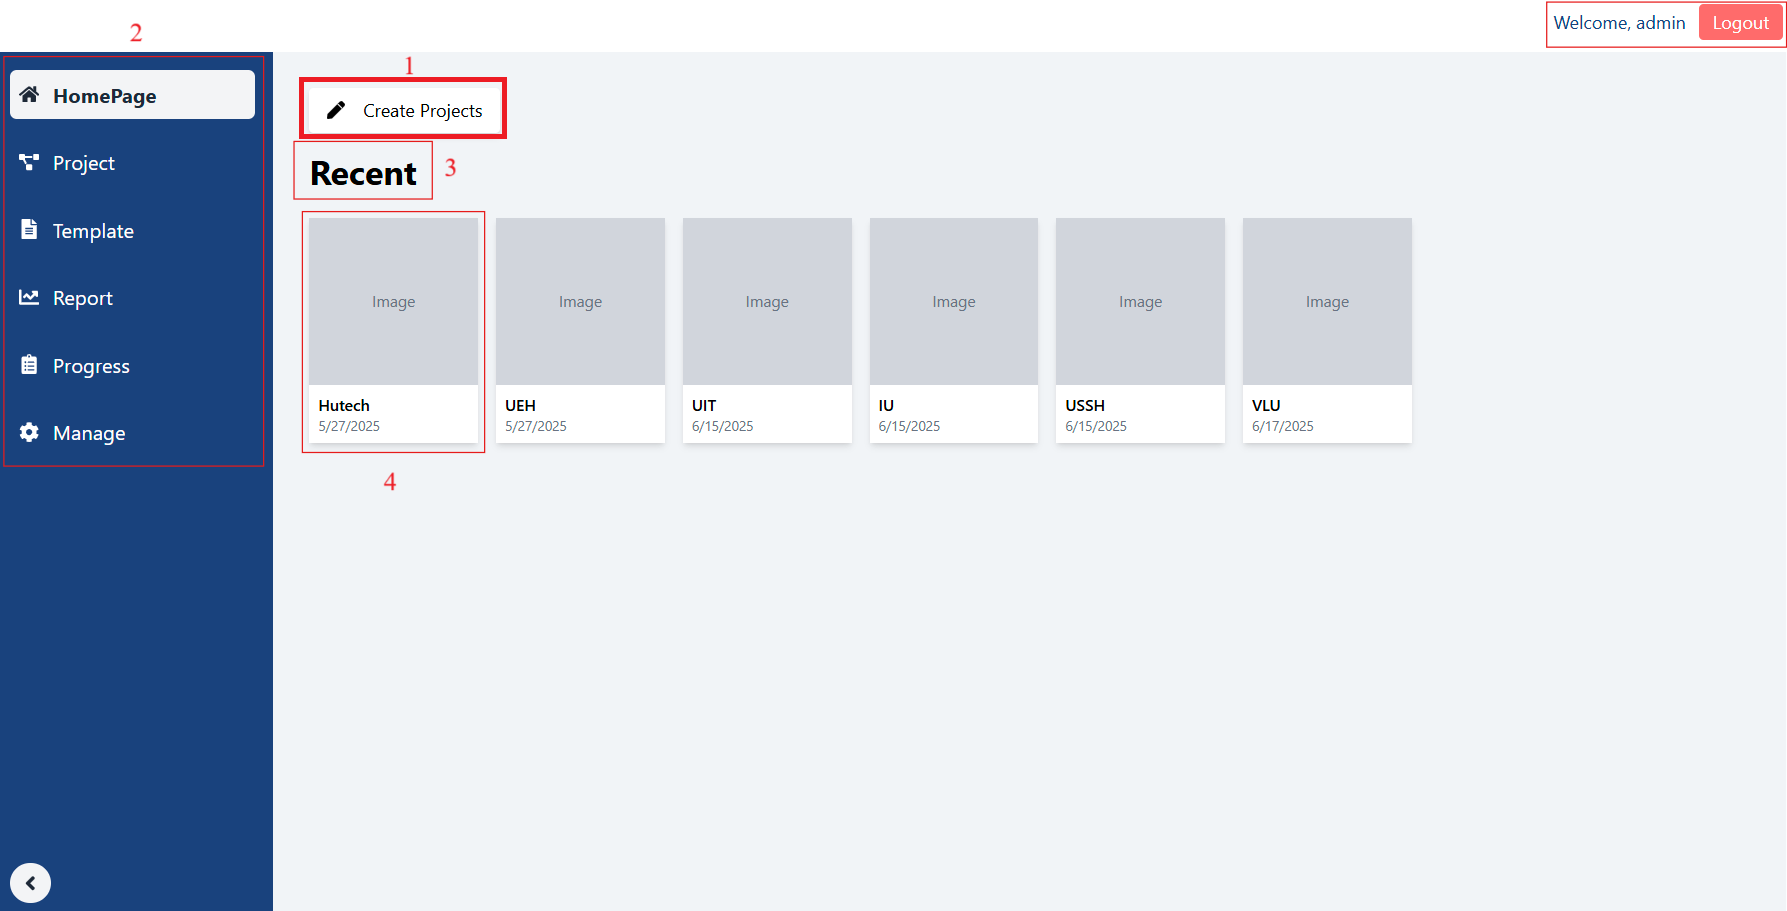
\includegraphics[width=1.2\textwidth]{images/homepage.png}
    \caption{Home page} 
    \label{fig:home}
\end{figure}
The homepage, as shown in Figure 4.1, represents the practical implementation outcome of the system’s administrator interface. This interface was developed to provide secretaries with a centralized and intuitive workspace for managing accreditation projects and related tasks.

The design includes a “Create Projects” button (point 1) positioned at the top of the page, enabling users to quickly initiate new projects. On the left side, a sidebar navigation menu (point 2) allows access to main modules, including Home page, Project, Template, Report, Progress, and Manage. This structure supports smooth navigation and aligns with the intended modular design of the application.

In the center of the page, the “Recent” section (point 3) displays recently created or updated projects, making it easier for administrators to continue work on active tasks. Below this, project cards (point 4) show basic information for each project, such as the institution name (e.g., Hutech, UEH, UIT) and the date of creation or last update. This design choice helps users quickly recognize and access ongoing projects.

\textbf{Steps to create new document from input template}

\begin{enumerate}
    \item To create a new accreditation document, the user first presses the “Create Projects” button, highlighted as point 1 in Figure 4.2. This action opens a form where the user can enter essential project information such as name, description, logo, members, status, and deadline.  
    \item After filling in the required input fields, the user continues by pressing the green “Create Project” button located at the bottom left corner of the form. Once the project is successfully created, the system automatically redirects the user to a Word-like workspace interface shown in Figure 4.3.
    \item At the top of this interface, there is a Select component which allows the user to choose from different predefined templates.
    \item When the user selects a specific template, its content is loaded into the document editor as demonstrated in Figure 4.4. From this point, the user can freely edit the document and has options to save, preview, or export the final version, thus supporting an efficient and streamlined accreditation report creation workflow.
\end{enumerate}

\begin{figure}[h]
\centering
    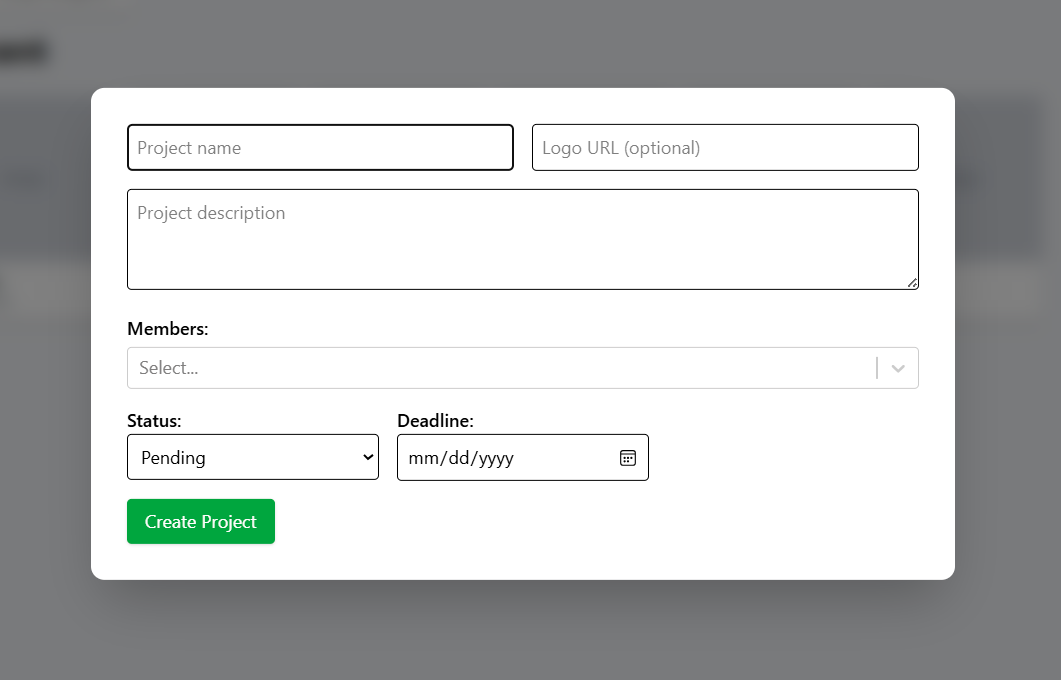
\includegraphics[width=0.5\textwidth]{images/create_process.png}
    \caption{The Project Creation Modal} 
    \label{fig:create_process}
\end{figure}
\begin{figure}[h]
\centering
    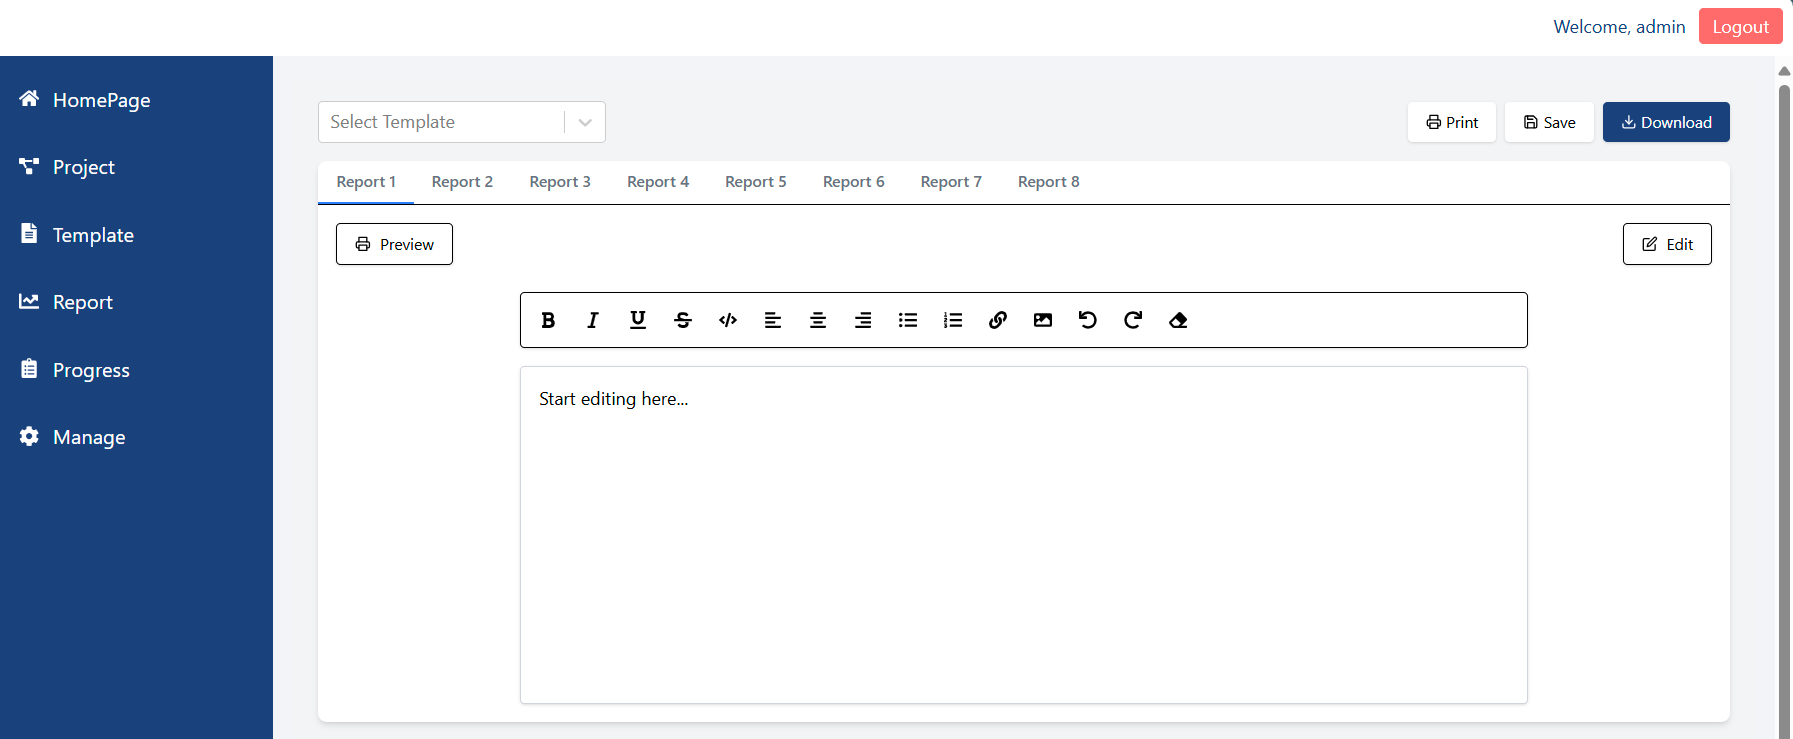
\includegraphics[width=1\textwidth]{images/empty_docs.png}
    \caption{The emty document page} 
    \label{fig:empty_docs}
\end{figure}
\begin{figure}[h]
\centering
    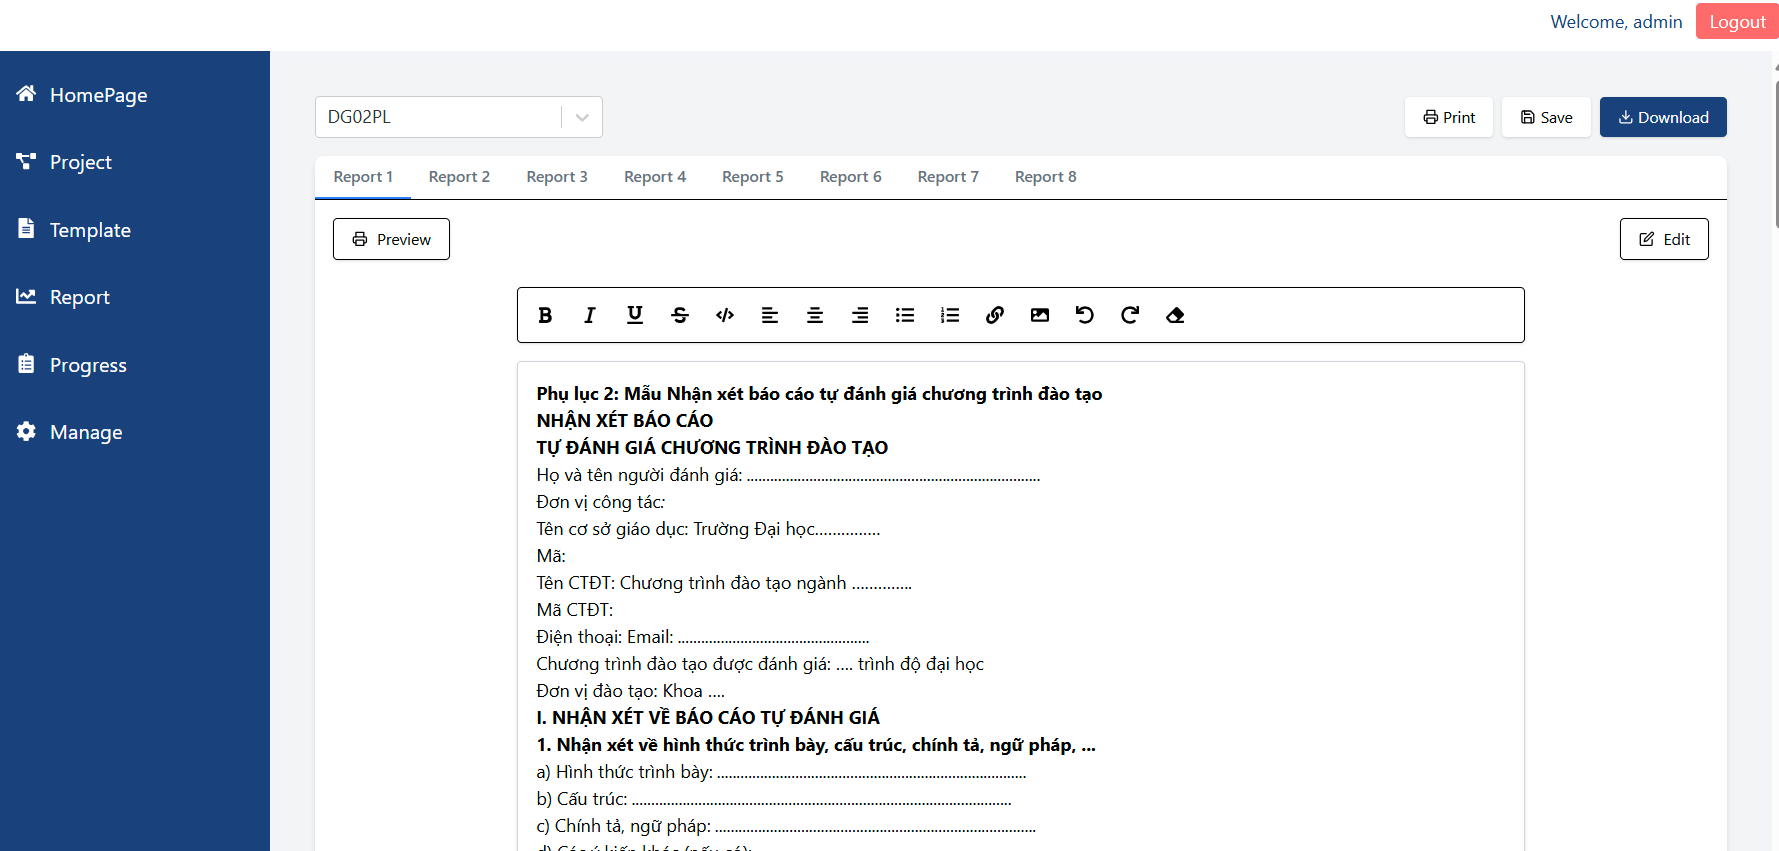
\includegraphics[width=1\textwidth]{images/complete_create.png}
    \caption{The document created by system according to the selected templates} 
    \label{fig:complete_create}
\end{figure}

\section{AI and LLMs model Result}
The refined PhoGPT was trained using a dataset collected from real accreditation documents and processed for Vietnamese context. After fine-tuning, the model achieved improvements in coherence, fluency, and relevance when generating suggestions or completing text.

Specifically, the refined model achieved:

\begin{enumerate}
    \item BLEU score: 26.5 (↑3.2 compared to base PhoGPT)
    \item ROUGE-L: 48.7 (↑4.1 compared to base PhoGPT)
    \item ROUGE-L: 48.7 (↑4.1 compared to base PhoGPT)
\end{enumerate}

Human evaluation: 86% of outputs were rated as relevant and useful by domain experts

This demonstrates that integrating domain-specific data significantly improves the model's performance in the specialized context of educational accreditation.
\section{Comparison}
When compared to related models and methods:

\begin{enumerate}
    \item Base PhoGPT: The original PhoGPT, trained on general Vietnamese text, performed well on everyday topics but lacked specificity and accuracy in educational accreditation language.
    \item PhoBERT: A transformer-based model focusing on understanding Vietnamese rather than generation, so it was less effective at generating full, context-aware recommendations.
    \itemm BART: Multilingual text generation showed reasonable performance but sometimes mixed non-Vietnamese tokens and lacked domain adaptation.
\end{enumerate}
    
Our refined PhoGPT, trained on domain-specific data, outperformed these models in generating accreditation-related text that aligns with official standards and professional tone. Unlike general models, the refined PhoGPT produced more coherent, formal, and contextually relevant suggestions tailored to the Vietnamese accreditation process.